\section{Социологический опрос}

Социалогический опрос молодого населения нашей страны был произведён с 
использованием современный технологий, представленные нам текущим развитием 
информационных технологий. Опросная анкета была составлена на базе проекта 
ИОМ <<Анкетолог>> (\url{http://anketolog.ru}) и проведена среди пользователей 
интернета. Сделана выборка из 300 анкет и проанализирована. Полученные данные 
представлены ниже.

В основном опрошены были молодые люди в возрасте от 18 до 29 лет, но с большим 
преобладанием лиц от 20 до 24 лет.

\begin{table}[H]
    \centering
    \begin{tabular}{|c|c|}
        \hline
        Возрастная группа, лет & Проценты \\ \hline \hline
        18 - 19 & 14 \\ \hline
        20 - 24 & 52 \\ \hline
        25 - 29 & 34 \\ \hline
    \end{tabular}
    \caption{Возрастные границы опрошенной группы}
    \label{table:01}
\end{table}

По половому признаку опрошенная группа разделилась, на 
\begin{table}[H]
    \centering
    \begin{tabular}{|c|c|}
        \hline
        Половой признак & Проценты \\ \hline \hline
        Мужской & 62,5 \\ \hline
        Женский & 37,5 \\ \hline
    \end{tabular}
    \caption{Половой признак опрошенной группы}
\end{table}

То есть можно сказать, что опрос был произведён по большей части у молодых 
лиц мужского пола.

Далее вопрос по полученному образованию разделился на такую группу
\begin{table}[H]
    \centering
    \begin{tabular}{|c|c|}
        \hline
        Образование & Проценты \\ \hline \hline
        Высшее & 30 \\ \hline
        Незаконченное высшее & 57,5 \\ \hline
        Среднее специально & 12,5 \\ \hline
    \end{tabular}
    \caption{Образование опрошенной группы}
\end{table}

Преобладание незаконченного высшего образования очевидно, исходя из анализа 
опрошенной возрастной группы, но присутствует небольшое расхождение с 
\ref{table:01}, но его можно считать незначительным.

Вопрос связанный с родом деятельности имеет множественный выбор. Данные между 
анкетируемыми распределились следующим образом:
\begin{table}[H]
    \centering
    \begin{tabular}{|c|c|}
        \hline
        Деятельность & Проценты \\ \hline \hline
        Студент университета & 69 \\ \hline
        Работаю & 31 \\ \hline
    \end{tabular}
    \caption{Основная деятельность группы}
\end{table}

То есть основная часть анкетируемых представляют студенты, но также нельзя не 
учитывать тот факт, что возможно и совмещение работы и учёбы.

Далее вопрос о доходе дал следующее результаты:
\begin{figure}[H]
    \centering
    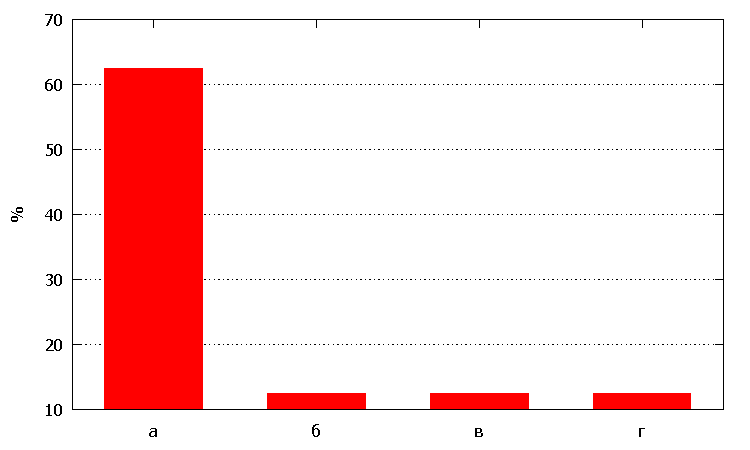
\includegraphics[width=0.8\textwidth]{work} \\
    \caption{Доход опрошенной группы. \\
        а -- достаточный на покупку необходимых 
        вещей (одежда, еда, лекарство)\\
        б -- испытываю трудности в покупке 
        необходимых вещей (одежда, еда, лекарство)\\
        в -- затрудняюсь ответить \\
        г -- другое 
    }
\end{figure}

В основном опрошенная группа лиц имеет достаточный доход, будь то работая 
дополнительно или на обеспечении у родителей. С этим пунктом всё придельно 
ясно, как никак основная масса опрошенных -- студенты.

По вопросу связанному с автомобилем основная часть опрошенных не имеет 
автомобиль в наличии (76\%), но у остальной группы в основном машина 
отечественного производства (18\%) и у остальной группы (4\%) иномарка. 
По этому поводу можно сказать одно -- не все студенты задумываются заранее 
обзавестись автомобилем (будь то материальные причины или какие-то другие 
обстоятельства), но можно предположить, что в более старшем возрасте эти 
показатели меняются в сторону с наличием машины.

Далее основная часть опроса связанная непосредственно с обсуждаемой проблемой.
\begin{table}[H]
    \centering
    \begin{tabular}{|c|c|c|}
        \hline
        Отношение & Разбогатели & Обеднели \\ \hline \hline
        С уважением & 12 & 4 \\ \hline
        С интересом & 10 & 2 \\ \hline
        С симпатией & 3 & 5 \\ \hline
        \textbf{Позитивное} & 25 & 11 \\ \hline \hline
        С подозрением, неприязнью & 19 & 3 \\ \hline
        С презрением & 5 & 2 \\ \hline
        С симпатией & 2 & 0 \\ \hline
        \textbf{Негативное} & 25 & 11 \\ \hline \hline
        Не лучше и не хуже, чем ко всем остальным & 44 & 67 \\ \hline
        Затрудняюсь ответить & 10 & 2 \\ \hline
        \textbf{Нейтральное} & 25 & 11 \\ \hline
    \end{tabular}
    \caption{<<Как вы относитесь к людям, которые разбогатели/обеднели?>>, \%}
\end{table}

Отношение к символу <<бедность>> существенно отличается от отношения к 
противоположному символу. Прежде всего -- две трети (67\%) опрошенных не 
имеют суждений по поводу <<бедности>>, и ещё 15\% затруднились ответить на 
этот вопрос. 

В отличие от богатых, обедневшие сограждане действительно вызывают у 
окружающих немного эмоций. Им, разумеется, никто не завидует, да и с симпатией 
относятся редко (5\%). Впрочем, для двух третей (67\%) опрошенных обедневшие 
люди ничем не лучше и не хуже остальных. 

Обратимся к следующему вопросу. 

Косвенным подтверждением высокой общественной ценности символа <<богатства>> в 
нашем обществе служит тот факт, что более половины опрошенных на вопрос: 
<<Что правит миром?>> ответили: деньги. Вторым по набранным результатам 
оказался разум (20\%), третим -- случай (11\%).

\begin{table}[H]
    \centering
    \begin{tabular}{|c|c|}
        \hline
        Вариант & Проценты \\ \hline \hline
        Деньги & 54 \\ \hline
        Разум & 20 \\ \hline
        Случай & 11 \\ \hline
        Любовь & 5 \\ \hline
        Высшая сила & 2 \\ \hline
        Случай & 3 \\ \hline
        Затрудняюсь ответить & 5 \\ \hline
    \end{tabular}
    \caption{<<Что по вашему мнению правит миром?>>, \%}
\end{table}

Вероятно, поляризация оценочных суждений о разбогатевших и обедневших людях 
происходит под влиянием контекста исследования, а не от того, что респонденты 
озабочены личностными качествами знакомых им богачей или бедняков. 

Называя качества, присущие богатым, респонденты ориентируются прежде всего 
на инструментальные ценности, с помощью которых, с их точки зрения, достигается 
богатство. Качествами, которыми <<вознаграждаются>> богатые, являются 
отклонениями от принятых в российском обществе <<стандартных>> человеческих 
характеристик. 

\newpage

\begin{table}[H]
    \centering
    \begin{tabular}{|c|c|c|}
        \hline
        Качества & Бедные & Богатые \\ \hline \hline
        Щедрость & 9 & 2 \\ \hline
        Жадность & 2 & 32 \\ \hline
        Доброта & 31 & 1 \\ \hline
        Чёрствость & 2 & 18 \\ \hline
        Инициативность, энергичность & 5 & 30 \\ \hline
        Пассивность, инертность & 21 & 2 \\ \hline
        Трудолюбие & 15 & 17 \\ \hline
        Лень & 22 & 4 \\ \hline
        Законопослушность & 28 & 2 \\ \hline
        Неуважение к закону & 2 & 26 \\ \hline
        Образованность & 9 & 21 \\ \hline
        Низкий уровень образования & 16 & 2 \\ \hline
        Совестливость & 19 & 1 \\ \hline
        Непорядочность & 1 & 21 \\ \hline
        Профессионализм & 5 & 19 \\ \hline
        Низкий уровень квалификации & 12 & 1 \\ \hline
        Патриотизм & 12 & 1 \\ \hline
        Безразличие к судьбе своей страны & 6 & 19 \\ \hline
        Не зависят & 32 & 31 \\ \hline
        Затрудняюсь ответить & 2 & 3 \\ \hline
    \end{tabular}
    \caption{<<Встречаются утверждения, что бедные и богатые различаются по 
        своим личным качествам. Отметьте не более пяти качеств, которые, 
        на ваш взгляд, в наибольшей степени присущи богатым/бедным?>>, \%}
\end{table}

Социальное значение символа <<бедность>> в современном российском обществе 
связано со страхами личность стать беспомощным в социальном и экономическом 
плане. 

Несправедливость общественного устройства, и прежде всего распределения 
материальных ценностей, считается основной причиной распространения бедности. 
В этом убеждены большинство. Среди конкретных причин называются несправедливо 
низкая оплата труда, низкий уровень пенсий и безработица и лень.

\begin{table}[H]
    \centering
    \begin{tabular}{|c|c|c|c|c|}
        \hline
        Явление & Всего & Хорошее & Среднее & Плохое \\ \hline \hline
        Несправедливая оплата труда & 59 & 43 & 59 & 64 \\ \hline
        Безработица & 39 & 26 & 39 & 43 \\ \hline
        Низкий уровень пенсий & 39 & 35 & 35 & 49 \\ \hline
        Злоупотребление спирт./нарк. & 34 & 28 & 36 & 33 \\ \hline
        Нежелание государства & 29 & 19 & 29 & 32 \\ \hline
        Недостаток средств на соц.помощь & 26 & 24 & 26 & 28 \\ \hline
        Несправедливое соц.устройство & 23 & 20 & 24 & 24 \\ \hline
        Лень & 21 & 20 & 24 & 24 \\ \hline
        Нехватка образования & 14 & 22 & 14 & 10 \\ \hline
        Низкий уровень нравственности & 13 & 11 & 13 & 13 \\ \hline
        Большой приток приезжих & 11 & 16 & 12 & 9 \\ \hline
        Однобокое развитие экономики & 11 & 7 & 12 & 11 \\ \hline
        Иждивенчество & 7 & 9 & 7 & 5 \\ \hline
        Большое число детей в семье & 5 & 7 & 5 & 4 \\ \hline
        Зависимое положении России & 4 & 6 & 4 & 4 \\ \hline
        Затрудняюсь ответить & 2 & 2 & 2 & 2 \\ \hline
        Другое & 1 & 1 & 1 & 1 \\ \hline
        Ничего из перечисленного & 0 & 0 & 0 & 0 \\ \hline
        Нет ответа & 0 & 0 & 0 & 0\\ \hline
    \end{tabular}
    \caption{<<Отметьте те явления, которые, по Вашему мнению, служат сейчас 
        основными причинами бедности в нашем обществе?>>, \%}
\end{table}

Устойчивой связи между жизненным успехом и символом <<богатство>>, а так же 
неуспехом и <<бедностью>>, которая присуща общественному сознанию западных 
стран, в российском общественном мнении пока нет. Тем не менее значение этих 
символом, особенно <<богатства>>, в определении характера социальной структуры 
очевидно. Состоятельные люди, крупные и средние предприниматели, элиты, 
успешные в разных сферах жизнедеятельности люди являются носителями символа 
<<богатство>> независимо от того, каково их реальное благосостояние, насколько 
широк ареал распространения их символического влияния -- страна, область, 
город, село. Представляется, что одна из задач современного общества 
заключается в том, чтобы осознать: носительство символа <<богатство>> 
возлагает высочайшую ответственность не только экономического характера и не 
может ограничиваться <<социально ответственностью бизнеса>> в виде честной 
уплаты налогов или благотворительности. От поведения этой социальной группы, 
от отношения большинства к ней зависят не только судьба рыночных отношений, 
но и стабильность общества, устойчивость социальной структуры. 

\begin{figure}[H]
    \centering
    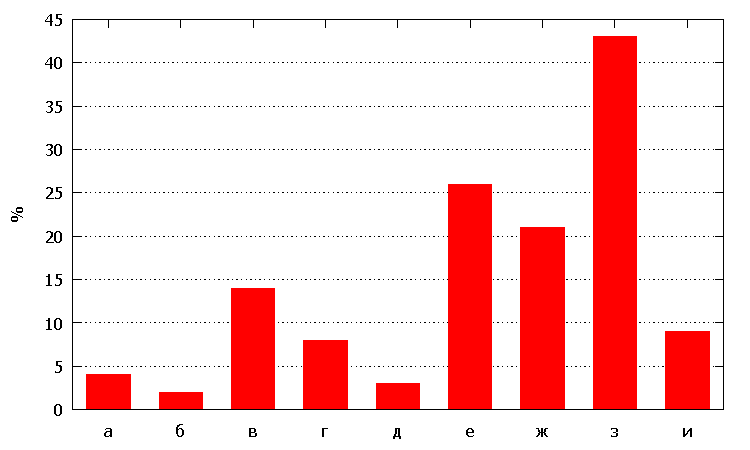
\includegraphics[width=1.0\textwidth]{statement} \\
    \caption{<<С какими из следующих суждений Вы бы прежде всего согласились?>> 
        \\
        а -- затрудняюсь ответить\\
        б -- другое \\
        в -- у меня вызывают подозрение люди с большими деньгами \\
        г -- я бы хотел(а) жить в обществе, где нет никаких денег \\
        д -- деньги не имеют для меня никакой ценности
        е -- для того чтобы жить нормально, нужно уметь планировать бюджет \\
        ж -- деньги, личное обогащение -- символ нашего времени \\
        з -- я испытываю уважение к людям, которые умеют делать деньги \\
        и -- я завидую людям, которые имеют много денег \\
    }
\end{figure}

Далее вопрос близкий по понятию, но акцентирующий роль на причинах социального 
неравенства в стране. Как очевидно это ни было, но в большинстве своём 
опрашиваемые склоняются к коррупции среди чиновников (75\%), далее идёт 
низкий уровень дохода (37.5\%) ну и остальные пункты равномерно распределились 
по (12.5\%).

\begin{figure}[H]
    \centering
    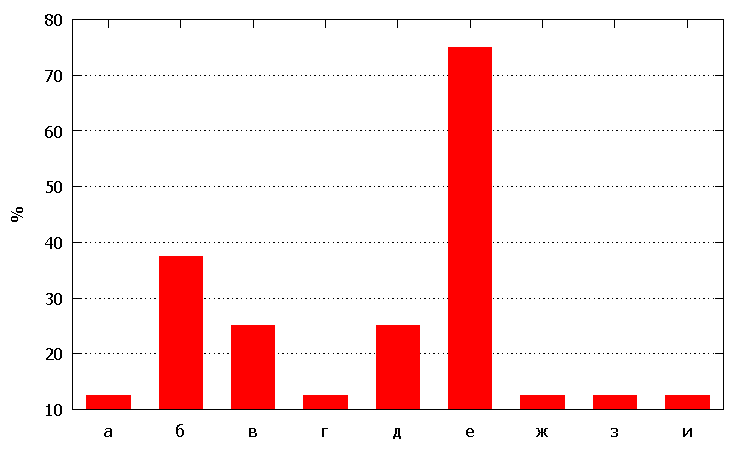
\includegraphics[width=1.0\textwidth]{reason} \\
    \caption{<<Назовите главную(ые), на Ваш взгляд, причину(ы) социального 
        неравенства.>> \\
        а -- высокий уровень инфляции \\
        б -- низкий уровень дохода \\
        в -- несправедливое распределение дохода \\
        г -- проводимая социальная политика \\
        д -- неэффективная работа правительства в социальной сфере \\
        е -- коррупция, взяточничество, воровство чиновников \\
        ж -- внешние обстоятельства, судьба, разные причины \\
        з -- затрудняюсь ответить \\
        и -- другое
    }
\end{figure}

Также вопрос из той же серии: <<Как вы считаете, какие основные причины 
социального неравенства?>>. Который только и подтверждает предыдущую диаграмму.
Лидером являются политические причины (50\%), далее идут экономические 
(37.5\%) и к другим причинам (12.5\%).

И последним завершающим вопросом является: <<Возможно ли на сегодняшний день 
улучшить свое положение в обществе?>>, где также большинство уверенно отвечает 
на него положительно, далее идёт <<скорее да, чем нет>> и самое минимальное 
значение у <<скорее нет, чем да>>.

Как известно, российское государство объявило борьбу с бедностью одним из 
приоритетов своей внутренней политики. В связи с этим было бы логично указать 
на то, что символические значения бедности и богатства могут и должны 
учитываться при выработке стратегии действий государства в этой сфере.

\newpage

\section*{Заключение}
\addcontentsline{toc}{section}{Заключение}

Во многих обществах распространён взгляд на бедность как на проявление зла и 
несправедливость, с которыми необходимо бороться. В российском обществе 
бедность пока не рассматривается в качестве социального врага. К сожаления, 
таково отношение скорее к богатству, а не к бедности. Поэтому, прежде чем 
выработать и приступить к реализации соответствующих реформ и мероприятий, 
важно направить усилия гражданского общества и государства на создание 
общественного мнения, благоприятствующего преодолению бедности -- объявление 
её <<вне закона>> и повышение престижа материального достатка. Тем самым будет 
заранее определена мировоззренческая база, с позиции которой государство и 
общество станут вести борьбу с бедностью, не забывая использовать 
стимулирующий к активному экономическому поведению фактор представлений о 
богатстве. Можно утверждать, что молодое поколение как и старшее довольно 
остро относится к данным социальным проблемам, поэтому они тоже могут играть 
немаловажную роль в становлении нашего общества.

\newpage